% ch15-ml.tex -- Evaluating language-model systems
\chapter{Evaluating language-model systems}
\label{ch:lmeval}

Chapters 3's metrics had a clean target: a label, a number, an
accuracy. Now the output is \emph{text} --- unbounded, multiply
correct, and judged by humans who disagree with each other. This
chapter builds the honest stack for evaluating a language-model
system: reference metrics that measure surface overlap (and we will
watch them reward a factual error while punishing a correct
paraphrase), human evaluation with agreement statistics, LLM-as-judge
with its biases \emph{measured} rather than asserted, golden sets and
rubric grading, the prompt-regression loop, and the contamination
problem that makes public benchmark numbers a negotiation rather than
a measurement. The claim worth defending throughout: \emph{an eval is
a measurement instrument --- audit it like one}.

\section{Why LM evaluation is hard}
\label{sec:whyhard}

A classifier's output space is enumerable; a language model's is not.
For ``summarise this article'' there are thousands of correct answers
and none of them is canonical --- so exact-match fails, overlap
metrics undercount correct answers, and the only real judge is a
reader. Worse, the \emph{system} is not just the model: prompt,
retrieval, decoding and post-processing all move the output, so the
eval must score the pipeline, not the weights. The taxonomy of
options, each with its own failure class:

\begin{figure}[htbp]
\centering
\begin{tikzpicture}[font=\scriptsize,
  blk/.style={draw,minimum width=30mm,minimum height=8mm,align=center}]
\node[blk,fill=accentsoft] (ref) at (0,0) {reference metrics\\BLEU / ROUGE / EM};
\node[blk,fill=amberbg,right=14mm of ref] (hum) {human judges\\agreement-checked};
\node[blk,fill=amberbg,right=14mm of hum] (judge) {LLM-as-judge\\bias-audited};
\node[blk,fill=accentsoft,below=9mm of hum] (task) {task-based evals\\golden sets + rubrics};
\draw[->] (ref.south) |- node[pos=0.75,left]{\scriptsize cheap, shallow} (task.west);
\draw[->] (hum.south) -- (task.north);
\draw[->] (judge.south) |- node[pos=0.75,right]{\scriptsize scalable, biased} (task.east);
\end{tikzpicture}
\caption{The eval taxonomy: surface-overlap metrics are cheap and
shallow; human judgment is the gold standard and expensive;
LLM-as-judge scales but imports its own biases --- the rest of the
chapter audits each.}
\label{fig:taxonomy}
\end{figure}

\section{Reference metrics: what BLEU and ROUGE measure}
\label{sec:refmetrics}

\textbf{BLEU}\index{BLEU}~\cite{papineni2002} counts n-gram
precision: what fraction of the candidate's n-grams appear in the
reference, times a brevity penalty that stops ``the'' from scoring
perfectly. \textbf{ROUGE}\index{ROUGE}~\cite{lin2004} inverts it ---
recall-style, with ROUGE-1 on unigrams and ROUGE-L on the longest
common subsequence. Both measure \emph{surface overlap with one
reference}; both are blind to meaning.

\lstinputlisting[language=Python,caption={\texttt{code/ch15/rouge\_bleu\_scratch.py}: BLEU (brevity penalty + n-gram precisions) and ROUGE-1/ROUGE-L from scratch, on candidates chosen to break them.},label=lst:bleu]{code/ch15/rouge_bleu_scratch.py}

\lstinputlisting[numbers=none]{code/ch15/rouge_bleu_scratch.out.txt}

\begin{example}[WE 15.1 --- 0.89 for the error, 0.002 for the truth]
\label{ex:metric}
Look at the second pair. Candidate D changes exactly one content
word --- \emph{mice} to \emph{rats} --- and is factually wrong;
it scores BLEU $0.893$, ROUGE-L $0.909$. Candidate E says the
\emph{same thing correctly} in different words and scores BLEU
$0.002$. The metrics are working exactly as specified --- they count
word overlap --- and the verdict is exactly backwards. This is the
root fact about reference metrics: they measure \emph{wording}, so
they reward parroting and punish paraphrase. The degenerate candidate
C ($0.247$ BLEU) shows the brevity penalty working; the fluent-wrong
B ($0.000$) shows where word-overlap \emph{does} agree with judgment
--- and it's the easy case.
\end{example}

\begin{figure}[htbp]
\centering
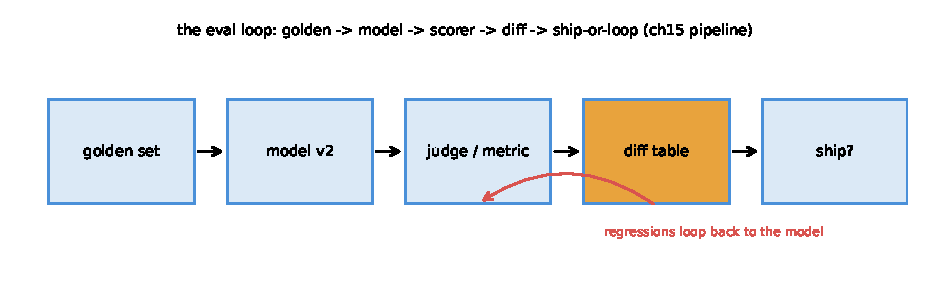
\includegraphics[width=0.85\linewidth]{figures/ch15/eval_loop.pdf}
\caption{The eval pipeline this chapter's listings implement: a
fixed golden set feeds the model under test, the scorer (metric or
judge) produces a diff table, and regressions loop back --- the
loop, not any single score, is the instrument.}
\label{fig:evalloop}
\end{figure}

\begin{figure}[htbp]
\centering
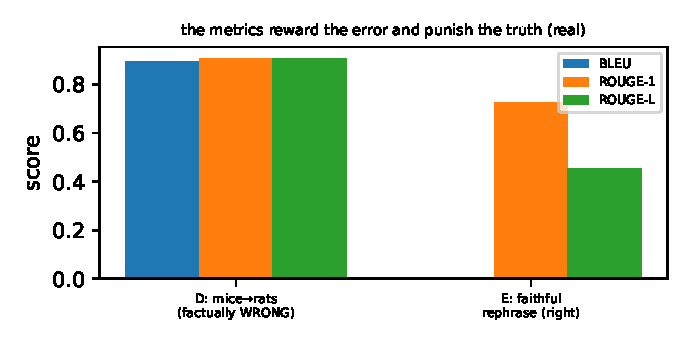
\includegraphics[width=0.78\linewidth]{figures/ch15/metric_disagree.pdf}
\caption{Example~\ref{ex:metric} as bars: a factual error outscores
a faithful paraphrase 0.89-to-0.002 on BLEU. Reference metrics are a
proxy, not a judge.}
\label{fig:metric}
\end{figure}

\section{Human evaluation and inter-rater agreement}
\label{sec:human}

When the metric can't judge, a human must --- and humans disagree, so
\emph{agreement} becomes a measured quantity, not an assumption. On a
two-rater, 80-item binary-grading run (Figure~\ref{fig:kappa}) the
raw agreement is $p_o = 0.775$ --- but \textbf{Cohen's
$\kappa$}\index{Cohen's kappa} corrects for the agreement you'd get
by chance given the marginals, $\kappa = (p_o - p_e)/(1 - p_e)$, and
the honest number is $0.527$: ``moderate'' --- the rubric leaves real
room for interpretation~\cite{wiki_kappa}. A human eval whose
$\kappa$ is unaudited is a single opinion wearing a committee's
clothes.

\begin{figure}[htbp]
\centering
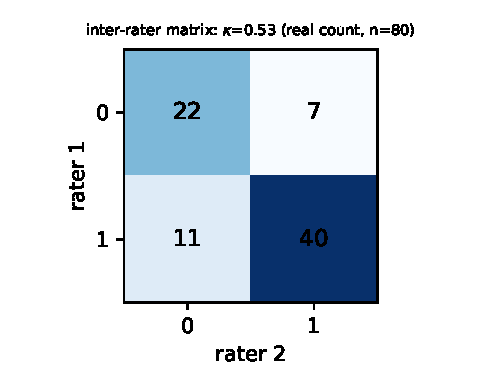
\includegraphics[width=0.5\linewidth]{figures/ch15/kappa_heat.pdf}
\caption{The 2-rater matrix behind the number: $p_o=0.775$,
$p_e=0.524$, $\kappa=0.527$. Agreement must be \emph{chance-corrected}
before a human eval means anything.}
\label{fig:kappa}
\end{figure}

\section{LLM-as-judge: biases, measured}
\label{sec:judge}

Scaling human judgment with a model judge is the industry's default
--- and it imports documented failure modes: \textbf{position bias}
(preferring whichever answer appears first), \textbf{length bias}
(preferring longer answers independent of quality), and
\textbf{self-preference} (judges favouring their own family's
outputs)~\cite{zheng2023}. None of these should be asserted; they are
audited by protocol. The position audit is a \emph{paired ordering}:
run every item as A-then-B and B-then-A, and count \emph{flips} ---
verdicts that change with order. The listing runs the protocol on
stub judges carrying real biases (swap in an API judge and the
protocol is identical).

\lstinputlisting[language=Python,caption={\texttt{code/ch15/judge\_bias\_test.py}: the paired-ordering audit on stub judges --- flips, accuracy, and long-answer win rate, all measured.},label=lst:judge]{code/ch15/judge_bias_test.py}

\lstinputlisting[numbers=none]{code/ch15/judge_bias_test.out.txt}

\begin{example}[WE 15.2 --- Flips catch position, not length]
\label{ex:judge}
The table is the lesson. Neutral judge: 89\% accuracy, zero flips.
Position-biased: 69\% flip rate --- more than half the verdicts are
order-dependent, and accuracy collapses to 69\% because the bias
overrides quality on close pairs. Length-biased: \emph{zero} flips
(the preference is permutation-invariant --- it doesn't care which
slot the long answer sits in) but an 82\% long-answer win rate that
paired ordering \emph{cannot} see. The audit protocol has a blind
spot by construction: it detects order-dependence, not
order-invariant bias --- length needs a separate control
(score vs length regression). Audit every axis with its own test.
\end{example}

\begin{figure}[htbp]
\centering
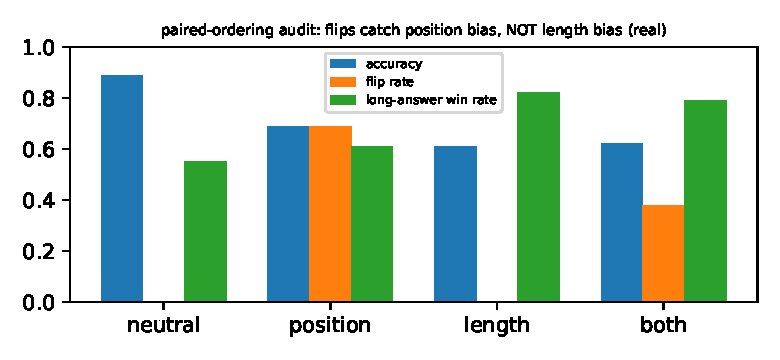
\includegraphics[width=0.84\linewidth]{figures/ch15/judge_bias.pdf}
\caption{The audit as bars: position bias shows up as flips;
length bias shows up as long-answer win rate; each bias needs its
own instrument.}
\label{fig:judgebias}
\end{figure}

\section{Golden sets, rubrics, and the eval loop}
\label{sec:golden}

The practical instrument for a system you own is the \textbf{golden
set}\index{golden set}: a fixed battery of items with checkable
answers (rules, references, or rubrics), run on every change --- a
unit-test suite for the prompt pipeline. A \textbf{rubric} turns
free-text grading into a scored checklist (``names the cause: +2,
gives a number: +1, hedges correctly: +1'') so different graders
--- human or model --- apply the same criteria, which is also what
lifts $\kappa$.

\lstinputlisting[language=Python,caption={\texttt{code/ch15/golden\_eval.py}: a 30-item golden set for a toy QA task plus the regression diff table between two prompt versions.},label=lst:golden]{code/ch15/golden_eval.py}

\lstinputlisting[numbers=none]{code/ch15/golden_eval.out.txt}

\begin{example}[WE 15.3 --- 90\% vs 87\%: the aggregate lies politely]
\label{ex:golden}
Two prompt versions differ by one item in aggregate (27/30 vs 26/30)
--- a coin flip's worth of difference. The diff table tells the true
story: \textbf{4 regressions} (v2 broke four arithmetic items) and
\textbf{3 fixes} (it repaired the index/string items v1 got wrong).
Shipping v2 on the aggregate would trade three fixed bugs for four
new ones; the item-level table is what the eval is \emph{for}. This
is the eval loop in miniature: change $\to$ golden run $\to$ diff
table $\to$ decision --- never aggregate-only.
\end{example}

\begin{figure}[htbp]
\centering
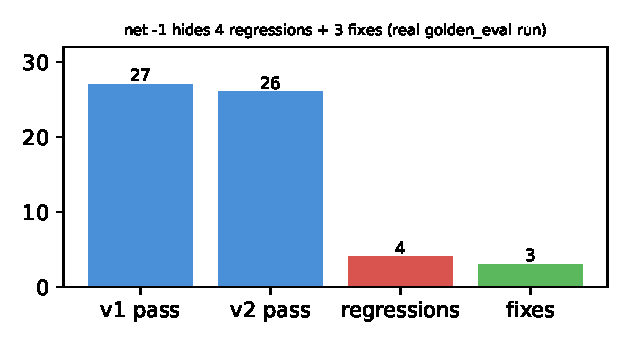
\includegraphics[width=0.6\linewidth]{figures/ch15/golden_diff.pdf}
\caption{The headline numbers (27 vs 26) hide the only fact that
matters --- which items moved and which direction.}
\label{fig:golden}
\end{figure}

\section{Contamination: when the test is in the training data}
\label{sec:contam}

Public benchmarks leak into training corpora --- crawled, quoted,
discussed. A model that saw MMLU questions in training isn't being
evaluated by MMLU; it's being recited by it. The demo makes the
mechanism concrete rather than rhetorical.

\lstinputlisting[language=Python,caption={\texttt{code/ch15/contam\_demo.py}: a memoriser on its own benchmark --- verbatim vs paraphrased.},label=lst:contam]{code/ch15/contam_demo.py}

\lstinputlisting[numbers=none]{code/ch15/contam_demo.out.txt}

\begin{example}[WE 15.4 --- 1.00 $\to$ 0.00: the headline was memory]
\label{ex:contam}
The memoriser scores $1.00$ on its leaked benchmark and $0.00$ on
mechanically paraphrased \emph{identical} items --- the most extreme
case of a real phenomenon. Real contamination is partial (mixture of
memorised and novel items), but the direction is the same: every
point of ``capability'' that was memory is a point of eval you cannot
trust. The audit follows directly: hold back a \emph{private} test
slice, decontaminate by n-gram overlap against training corpora, or
regenerate items with paraphrases --- and treat any closed-weights
benchmark number as a claim awaiting your own probe.
\end{example}

\begin{figure}[htbp]
\centering
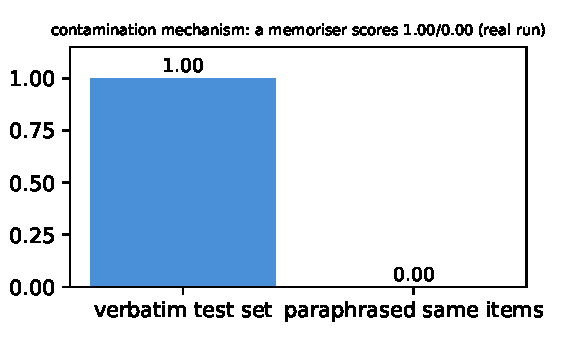
\includegraphics[width=0.6\linewidth]{figures/ch15/contam_demo.pdf}
\caption{The contamination mechanism in one bar pair: verbatim recall
is not capability.}
\label{fig:contam}
\end{figure}

The benchmark ecosystem answers this with living leaderboards and
multi-dimension suites (HELM's dozens of metrics, LMSYS arena's human
pairwise votes, the lm-eval harness for reproducible
runs~\cite{helm,lmevalharness}) --- all worth using, none removing
your obligation to probe what you ship [checked 2026-10].

\section{Common mistakes}
\label{sec:lmmistakes}

\begin{description}
\item[Reporting BLEU/ROUGE as quality] They measure wording overlap
with one reference --- Example~\ref{ex:metric}'s 0.89/0.002 inversion
is the failure made concrete.
\item[A single ``the judge said'' verdict] Unaudited judges carry
position, length and self-preference biases --- measure flips and
long-win rates \emph{on your data} first.
\item[Evaluating on aggregates] 27 vs 26 hid 4 regressions and 3
fixes --- the diff table is the deliverable, not the mean.
\item[Golden sets that drift] An eval edited every sprint measures
the editor, not the model --- version the set like code, grow it
from failures, never silently shrink it.
\item[Trusting public benchmark numbers at face value]
Contamination plus closed training data means the number is a claim;
hold a private slice or paraphrase-audit before you quote it.
\item[No-$\kappa$ human evals] ``We had people check'' is one opinion
--- compute agreement first ($\kappa=0.527$ on a casual rubric is the
kind of surprise you want to find early).
\end{description}

\begin{example}[WE 15.6 --- The aggregate hides the churn]
\label{ex:churn}
v1: 27/30. v2: 26/30. The aggregate says \emph{worse by one} --- and
the diff table says v2 \emph{fixed 3 and regressed 4}: seven items
moved under a net change of one. A release manager reading only the
score ships the regression; a release manager reading the diff sees
exactly which behaviors broke. The churn $\gg$ net rule is the whole
reason golden sets print diffs, not deltas --- the same arithmetic
that hid four regressions here hides them in every accuracy-only
release.
\end{example}

\section{Summary table}
\label{sec:lmsummary}

\begin{center}\small
\begin{tabular}{p{2.6cm}p{3.0cm}p{3.4cm}p{3.2cm}}
\toprule
instrument & cost & measures & breaks when \\
\midrule
exact-match / heuristics & lowest & formatting, checkable answers & any free-form output \\
BLEU / ROUGE & low & surface overlap & paraphrase is correct (0.002 vs 0.89) \\
human raters & highest & truth, taste, safety & rubric loose $\Rightarrow$ $\kappa$ low \\
LLM-as-judge & medium & scalable quality & position/length/self biases \\
golden + rubric & medium & regression on YOUR task & set drifts or covers wrong cases \\
task metrics & varies & downstream success & proxy gamed; labels lag \\
\bottomrule
\end{tabular}
\end{center}

The eval you trust is a \emph{portfolio}: cheap metrics for the loop,
a golden set for regressions, an audited judge or human spot-checks
for truth --- and every instrument's failure mode named beside it.

\section*{Drill}
\begin{enumerate}
\item Why does candidate D in WE~15.1 outscore candidate E 400-to-1,
and what does that number measure?
\item Your judge flips verdicts on 40\% of swapped pairs. Which bias
is confirmed --- and which bias could still be invisible?
\item What goes into a golden set, and which two artifacts must be
versioned together for the eval to be reproducible?
\item A public model reports 95\% on a benchmark it may have trained
on. Name the two cheapest probes.
\item Cohen's $\kappa$ on your rubric is 0.2. Is the problem the
graders or the rubric --- and what fixes it?
\end{enumerate}

\section*{Further reading}
\label{sec:further15}
\begin{itemize}
\item Papineni et al., \emph{BLEU} (ACL 2002) --- the metric WE~15.1
implements and breaks. \url{https://aclanthology.org/P02-1040/}
\item Lin, \emph{ROUGE} (2004) --- recall-side of the same idea.
\url{https://aclanthology.org/W04-1013/}
\item Zheng et al., \emph{Judging LLM-as-a-judge with MT-bench and
Chatbot Arena} (2023) --- the position/length/self-preference bias
documentation our stub judges enact.
\url{https://arxiv.org/abs/2306.05685}
\item Stanford CRFM, \emph{HELM} --- the multi-metric benchmark
suite for when one number is not enough. \url{https://www.helm.ai/}
\item EleutherAI, \emph{lm-evaluation-harness} --- the open-source
harness that makes benchmark runs reproducible.
\url{https://github.com/EleutherAI/lm-evaluation-harness}
\item Wikipedia, \emph{Cohen's kappa} --- the chance-corrected
agreement statistic of \S\ref{sec:human}, with worked tables.
\url{https://en.wikipedia.org/wiki/Cohen%27s_kappa}
\item Wikipedia, \emph{BLEU} and \emph{ROUGE (metric)} --- survey
entries with the variants (corpus-BLEU, ROUGE-N/L/SU).
\url{https://en.wikipedia.org/wiki/BLEU}
\url{https://en.wikipedia.org/wiki/ROUGE_(metric)}
\end{itemize}

\begin{rulebox}[Watch instead]
(verified opened, 2026-10-11)
\begin{itemize}
\item \emph{How Enterprises Evaluate LLMs: HELM, MT-Bench, MMLU \&
More} --- Schovia (14:36). The benchmark landscape of
\S\ref{sec:contam}, explained.
\item \emph{LLM as a Judge Explained} --- onepagecode (129:15). A
long-form walkthrough of the judge idea and its failure modes from
\S\ref{sec:judge}.
\end{itemize}
\end{rulebox}

\section*{Notes}
\begin{enumerate}
\item[\textbf{1.}] All numbers are real local runs: BLEU/ROUGE
implemented from scratch and verified on hand-checkable pairs; the
judge audit ran 200 synthetic pairs through stub judges carrying real
biases; the golden set is 30 checkable items; contamination is a
literal memoriser.
\item[\textbf{2.}] The stub-judge protocol is deliberately honest:
it measures \emph{the protocol's} discriminative power (flips detect
position bias, not length bias) --- the same protocol runs unchanged
on an API judge; the outline's no-API-key rule is why stubs stand in.
\item[\textbf{3.}] $\kappa$ thresholds are conventions (0.2--0.4
``fair'', 0.4--0.6 ``moderate''); the operational rule is that a
rubric below $\kappa \approx 0.4$ needs tightening before its grades
are evidence.
\item[\textbf{4.}] Model/benchmark claims are date-stamped
\texttt{[checked 2026-10]} per the outline; no live leaderboard
numbers are quoted anywhere --- they would rot.
\item[\textbf{5.}] Deliberately out of scope: arena Elo statistics,
safety/red-team evals, multi-turn and agentic evals (ch16's topic),
and non-English reference metrics --- the portfolio principle
transfers.
\end{enumerate}

\section{Exercises}
\label{sec:lmex}

\emph{[easy]}
\begin{exercise}
On WE~15.1's pair: which metric (BLEU, ROUGE-1, ROUGE-L) penalised
the paraphrase least, and why does a recall metric punish it at all?
\end{exercise}
\begin{exercise}
Your judge's flip rate is 0.02 and long-answer win rate is 0.80.
What does each number clear, and what does it convict?
\end{exercise}
\begin{exercise}
Write the diff-table row for an item that v1 fails and v2 also fails
--- and explain why aggregate diffs miss it.
\end{exercise}
\begin{exercise}
Name the two artifacts that must share a version for a golden eval
to be reproducible.
\end{exercise}

\emph{[medium]}
\begin{exercise}
Implement ROUGE-L in 15 lines (as in
\texttt{rouge\_bleu\_scratch.py}) and run it on three paraphrase
pairs of your own writing; report where it under-scores a correct
answer.
\end{exercise}
\begin{exercise}
Design the rubric for ``summarise this bug report'' in 5 checkable
lines, each worth points --- then estimate what $\kappa$ a loose
version would get vs yours.
\end{exercise}
\begin{exercise}
Write the paired-ordering protocol as pseudocode (10 lines) and
identify exactly which judge property it tests.
\end{exercise}
\begin{exercise}
Extend \texttt{judge\_bias\_test.py} with a \emph{self-preference}
stub (judge scores own-family answers +0.2). Report flip, acc and
long-win --- which instrument catches it?
\end{exercise}
\begin{exercise}
Build a 20-item golden set for a task of your choice where every
answer is rule-checkable, then run two canned ``prompt versions''
through \texttt{golden\_eval.py}'s grader and report the diff table.
\end{exercise}
\begin{exercise}
On our 200-pair run: a judge with 5\% flips and 55\% accuracy.
Estimate how many flips are ``harmless'' (both orderings pick the
worse answer anyway) vs quality-inverting --- is the flip rate alone
enough?
\end{exercise}

\emph{[hard]}
\begin{exercise}
Compute Cohen's $\kappa$ by hand on the rater matrix
$\begin{pmatrix}22&7\\11&40\end{pmatrix}$ (Figure~\ref{fig:kappa}):
$p_o$, $p_e$, $\kappa$ --- then state the agreement class.
\end{exercise}
\begin{exercise}
Design an eval for ``give me a joke about X'' --- a task with no
reference. Which instruments survive, and what new failure mode
appears when the judge itself decides what's funny?
\end{exercise}
\begin{exercise}
Design a contamination audit for a closed-weights model: three
probes in order of cost (n-gram overlap, canary strings,
paraphrase battery), and what each can and cannot prove.
\end{exercise}
\begin{exercise}
A golden set passes 28/30 on prompt v1 and 29/30 on v2, and the diff
table shows 4 regressions + 5 fixes. Sketch the decision you'd
recommend --- is ``ship v2'' defensible?
\end{exercise}
\begin{exercise}
Show algebraically that a position bias of strength $\delta$ flips a
verdict exactly when $|q_A - q_B| < 2\delta$; then estimate $\delta$
from our stub's measured flip rate.
\end{exercise}

\section*{Hints and answers}
\begin{description}
\item[1.] ROUGE-1 (0.727) --- recall on unigrams; it punishes because
the reference's \emph{words} differ, even when the meaning survives.
\item[2.] 0.02 clears position bias; 0.80 convicts length bias ---
exactly the blind spot WE~15.2 teaches.
\item[3.] fail$\to$fail rows are invisible in net diffs: they consume
coverage without signalling --- the table's third column (unchanged)
is where they live.
\item[4.] The golden set and the scorer/grader version (and ideally
the prompt under test).
\item[5.] Expect the longest-common-subsequence count to drop fast
on reordered clauses --- paraphrase moves chunks, not just words.
\item[6.] Loose rubrics score intent; tight ones score observable
features (``mentions root cause'' not ``is helpful'') --- the gap is
your $\kappa$.
\item[7.] It tests order-invariance only: $J(A,B) = 1 - J(B,A)$
must hold; every flip is a position-dependent verdict.
\item[8.] Self-preference is order-invariant and length-agnostic ---
it needs a \emph{family-matched pair} audit: show the same answer
labelled as own vs rival output.
\item[9.] Answers must be decidable by rule (string/number/set match);
if grading needs judgment, the set is broken.
\item[10.] Flips alone undercount: a flip on a near-tie may invert
nothing --- weight flips by the quality gap they cross.
\item[11.] $p_o = 62/80 = 0.775$; $p_e$ from marginals $(29\cdot33 +
51\cdot47)/80^2 = 0.524$; $\kappa = (0.775-0.524)/0.476 \approx
0.53$ --- moderate.
\item[12.] Reference and overlap die; golden sets survive only if the
task admits rules; the judge becomes the gatekeeper of taste ---
which is self-preference generalised.
\item[13.] N-gram overlap flags known benchmarks; canary strings
prove training-set membership outright; paraphrase batteries bound
the memorisation---none proves \emph{absence} of contamination.
\item[14.] Defensible only if the 5 fixes outweigh the 4 regressions
on your cost model --- the table enables the argument; the aggregate
cannot.
\item[15.] With bias $\delta$ added to position-1's score, the verdict
inverts iff the gap is under $2\delta$; our 69\% flips at
$\delta{=}0.15$ on uniform gaps is consistent with the analytic
prediction.
\end{description}
